\documentclass[10pt, letterpaper]{article}
\usepackage{setspace}
\usepackage[letterpaper, margin=1.0in]{geometry}
\addtolength{\topmargin}{-0.25in}
%\usepackage{tocloft}
\usepackage{titlesec}
%\titleformat*{\section}{\large\bfseries}
\titleformat*{\section}{\large}
\titleformat*{\subsection}{\normalsize}
\usepackage{enumitem}
\usepackage{listings}
\usepackage{amsmath}   % includes \boldmath(), \boldsymbol{()}
\usepackage{bm}        % math fonts, \boldmath{}, \boldsymbol{}
\usepackage{graphicx}
\usepackage{float}
\graphicspath{{images/}}
\usepackage{subcaption}
\usepackage{xcolor, colortbl}
\definecolor{gray}{gray}{0.9}
\definecolor{ltBlue}{rgb}{0.75, 0.85, 0.975}
\definecolor{medBlue}{rgb}{0.75, 0.8, 0.9}
\definecolor{white}{rgb}{1, 1, 1}
%\rowcolor{ltBlue}
\usepackage{changepage}
\usepackage{pdflscape}
\bibliographystyle{plainnat}
\usepackage[authoryear, round, semicolon]{natbib}
\newcommand{\mt}[1]{\bm{#1}^{\prime}}
\newcommand{\mtm}[2]{\bm{#1}^{\prime}\bm{#2}}
\newcommand{\mi}[1]{\bm{#1}^{-1}}
\newcommand{\mest}[1]{\hat{\bm{#1}}}
\usepackage[bottom]{footmisc}
\setlength{\skip\footins}{12pt}
\setlength\parindent{0pt}
%\usepackage{breakurl}
\usepackage{url}
\usepackage{hyperref}
\hypersetup{
    colorlinks=true,
    linkcolor=blue,
    urlcolor=blue,
}
% Disable section numbers, so that hyperlinks are enabled
%\setcounter{secnumdepth}{0}

\title{\Large Co-lab Shiny Workshop\\[6pt]
       \large Integrating Shiny and \texttt{plotly}\\[6pt]
       November 5, 2020\\[20pt]
       \normalsize thomas.balmat@duke.edu\\[1pt]rescomputing@duke.edu}

%\date{\vspace{-30pt}October 17, 2019}
\date{}
%\author{thomas.balmat@duke.edu\\rescomputing@duke.edu}

\begin{document}
    
\begin{spacing}{1.0}
    
\maketitle

\vspace{-20pt}

%%%%%%%%%%%%%%%%%%%%%%%%%%%%%%%%%%%%%%%%%%%%%%%%%%%%%%%%%%%%%%%%%%%%%%%%%%%%%%%%%%%%%%%%%%%%

In previous sessions of the series, we used features of Shiny, \texttt{Data Tables}, and \texttt{ggplot} to accept input from a visitor to your site and, in the context of analyses implemented, present informative results intended to guide the analyst through further exploration of a data set.  One strength of an app developed in  Shiny is that analyses, tables, and graphs are prepared with no requirement from the user other than to ``fill out" the input form and wait a moment for results to appear.  The ease of iterative adjustment of on-screen controls and review of results promotes idea generation and validation, making a well designed Shiny app a resource for exploratory data research.  In this session, we will use \texttt{plotly} to add hover labels and clickable geoms to a \texttt{ggplot} graph, making it more dynamic through filtering, highlighting, and updating of views as the user probes visible features and relationships in the data.  Because we are using \texttt{plotly} in a Shiny context, our emphasis will be on the interaction of \texttt{plotly} features and functions with your Shiny script, particularly within the \texttt{server()} function.


%%%%%%%%%%%%%%%%%%%%%%%%%%%%%%%%%%%%%%%%%%%%%%%%%%%%%%%%%%%%%%%%%%%%%%%%%%%%%%%%%%%%%%%%%%%%

\section{Overview}

\begin{itemize}
    \item Preliminaries
      \begin{itemize}
        \item What can Shiny and \texttt{plotly} do for you?
        \item What are your expectations of this workshop?
      \end{itemize}
    \item \hyperref[sec:examples]{Examples}
    \item \hyperref[sec:resources]{Resources}
    \item \hyperref[sec:anatomyofapp]{Anatomy of a Shiny app}
    \item \hyperref[sec:accesworkshopmaterial]{Workshop material}
    \item \hyperref[sec:prevapps]{Review apps from previous sessions}
      \begin{itemize}
          \item \hyperref[sec:prevappOPM]{\texttt{Data Tables} and \texttt{ggplot}: Office of Personnel Management Human Capital analysis}
          \item \hyperref[sec:prevappfltmap]{More \texttt{ggplot}: U.S. domestic flight map}
      \end{itemize}
    \item \hyperref[sec:hello]{Hello \texttt{plotly}}
    \item \hyperref[sec:pleiotropy]{\texttt{plotly} app:  GWAS pleiotropy}
    \item \hyperref[sec:debugging]{Debugging}
\end{itemize}

% Shiny server
% http vs. https
% Global mem

%%%%%%%%%%%%%%%%%%%%%%%%%%%%%%%%%%%%%%%%%%%%%%%%%%%%%%%%%%%%%%%%%%%%%%%%%%%%%%%%%%

\section{Examples}\label{sec:examples}

\begin{itemize}[noitemsep]
  \item \texttt{plotly} Visualizations
    \begin{itemize}
      \item \texttt{plotly} gallery:  \url{https://plot.ly/r/shiny-gallery/}
      \item Frank Harrell
        \begin{itemize}
          \item More with less:  \url{https://www.fharrell.com/post/interactive-graphics-less/}
          \item Hmisc package:  \url{https://cran.r-project.org/web/packages/Hmisc/Hmisc.pdf}
          \item Recent presentation:  \url{http://hbiostat.org/talks/rmedicine19.html}
        \end{itemize}
    \end{itemize}
  \item Shiny Apps
    \begin{itemize}[noitemsep]
      \item Duke Data+ project:  \textit{Big Data for Reproductive Health}, \url{http://bd4rh.rc.duke.edu:3838}
      \item Duke Med H2P2 Genome Wide Association Study:  \url{http://h2p2.oit.duke.edu}
    \end{itemize}
\end{itemize}


%%%%%%%%%%%%%%%%%%%%%%%%%%%%%%%%%%%%%%%%%%%%%%%%%%%%%%%%%%%%%%%%%%%%%%%%%%%%%%%%%

\section{Resources}\label{sec:resources}

\begin{itemize}

  \item R
    \begin{itemize}   
      \item Books
        \begin{itemize}[noitemsep]
          \item Norm Matloff, \textit{The Art of R Programming}, No Starch Press
          \item Wickham and Grolemund, \textit{R for Data Science}, O'Reilly
          \item Andrews and Wainer, \textit{The Great Migration:  A Graphics Novel}, \url{https://rss.onlinelibrary.wiley.com/doi/pdf/10.1111/j.1740-9713.2017.01070.x}
          \item Friendly, \textit{A Brief History of Data Visualization}, \url{http://datavis.ca/papers/hbook.pdf}
        \end{itemize}
      \item Reference cards
        \begin{itemize}[noitemsep]
          \item R reference card:  \url{https://cran.r-project.org/doc/contrib/Short-refcard.pdf}
          \item Base R:  \url{https://rstudio.com/wp-content/uploads/2016/10/r-cheat-sheet-3.pdf}
          \item Shiny, \texttt{ggplot}, \texttt{markdown}, \texttt{dplyr}, \texttt{tidy}: \url{https://rstudio.com/resources/cheatsheets/}
          \item \texttt{plotly}: \url{https://plotly.com/r/reference/}
        \end{itemize}
    \end{itemize}

  \item Shiny
    \begin{itemize}[noitemsep]
        \item \texttt{?shiny} from the R command line
        \item Click \texttt{shiny} in the \texttt{Packages} tab of RStudio
        \item \url{https://cran.r-project.org/web/packages/shiny/shiny.pdf}
    \end{itemize}

  \item \texttt{plotly}
    \begin{itemize}[noitemsep]
        \item \texttt{?plotly} from the R command line
        \item Click \texttt{plotly} in the \texttt{Packages} tab of RStudio
        \item \url{https://cran.r-project.org/web/packages/plotly/plotly.pdf}
    \end{itemize}

  \item Workshop materials
    \begin{itemize}
        \item \url{https://github.com/tbalmat/Duke-Co-lab/tree/master/Session-4}
    \end{itemize}
\end{itemize}

%%%%%%%%%%%%%%%%%%%%%%%%%%%%%%%%%%%%%%%%%%%%%%%%%%%%%%%%%%%%%%%%%%%%%%%%%%%%%%%%%%%%%%%%%%%%%%

\section{Anatomy of a Shiny App}\label{sec:anatomyofapp}

A Shiny app is an R script executing in an active R environment that uses functions available in the Shiny package to interact with a web browser.  The basic components of a Shiny script are

\begin{itemize}
    \item \texttt{ui()} function
    \begin{itemize}
        \item Contains your web page layout and screen objects for inputs (prompt fields) and outputs (graphs, tables, etc.)
        \item Is specified in a combination of Shiny function calls and raw HTML
        \item Defines variables that bind web objects to the execution portion of the app
    \end{itemize}
    \item \texttt{server()} function
    \begin{itemize}
        \item The execution portion of the app
        \item Contains a combination of standard R statements and function calls, such as to \texttt{apply()}, \texttt{lm()}, \texttt{ggplot()}, etc., along with calls to functions from the Shiny package that enable reading of on-screen values and rendering of results
    \end{itemize}
    \item \texttt{runApp()} function
    \begin{itemize}
        \item Creates a process listening on a tcp port, launches a browser (optional), renders a screen by calling the specified \texttt{ui()} function, then executes the R commands in the specified server() function
    \end{itemize}
\end{itemize}

%%%%%%%%%%%%%%%%%%%%%%%%%%%%%%%%%%%%%%%%%%%%%%%%%%%%%%%%%%%%%%%%%%%%%%%%%%%%%%%%%%%%%%%%%%%%%%

\section{Access Workshop Material}\label{sec:accesworkshopmaterial}

Repository:  \url{https://github.com/tbalmat/Duke-Co-lab}

\begin{itemize}[noitemsep]
    \item Previous session (\texttt{Data Tables}):  \url{https://github.com/tbalmat/Duke-Co-lab/tree/master/Session-2}
    \item Previous session (\texttt{ggplot}):  \url{https://github.com/tbalmat/Duke-Co-lab/tree/master/Session-3}
    \item Current session (\texttt{plotly}):  \url{https://github.com/tbalmat/Duke-Co-lab/tree/master/Session-4}
\end{itemize}

Execute locally:

\begin{itemize}
    \item Download and expand (in separate local directories) zip file(s) from \url{https://github.com/tbalmat/Duke-Co-lab}, session-2, session-3, and session-4 directories, or download individual script and data files as needed
    \item Edit R source files (\texttt{CPDFTables.r}, \texttt{FlightEvaluation.r}, \texttt{Pleiotropy.r}, \texttt{ui.r}, \texttt{server.r}) and modify \texttt{setwd()} instructions to target directories on your computer
    \item Launch RStudio
    \item Install Shiny packages (execute following at R command prompt):
    \begin{itemize}[noitemsep]
        \item \texttt{install.packages("shiny")}
        \item \texttt{install.packages("shinythemes")}
        \item \texttt{install.packages("ggplot2")}
        \item \texttt{install.packages("maps")}
        \item \texttt{install.packages("ggridges")}
        \item \texttt{install.packages("ggrepel")}
        \item \texttt{install.packages("plotly")}
    \end{itemize}
    \item Execute R script(s) (\texttt{CPDFTables.r}, \texttt{FlightEvaluation.r}, \texttt{Pleiotropy.r})
\end{itemize}


%%%%%%%%%%%%%%%%%%%%%%%%%%%%%%%%%%%%%%%%%%%%%%%%%%%%%%%%%%%%%%%%%%%%%%%%%%%%%%%%%%%%%%%%%%%%%%

\section{Review apps from previous sessions}\label{sec:prevapps}

The example app for current session uses a single control (a statistical significance level) to filter observations to be selected for plotting.  Before proceeding we should review previous apps, which involved many more controls and interacted with R scripts in a number of ways.  As we review the example app today, try to imagine how we might incorporate additional controls and techniques employed in previous apps. 

\subsection{\texttt{Data Tables} and \texttt{ggplot()}: Office of Personnel Management Human Capital analysis}\label{sec:prevappOPM}

Features of interest:

\begin{itemize}[noitemsep]
    \item Use of tabs and side bar panels to organize app
    \item Use of notification window for status reporting
    \item Use off cascading style sheets
    \item Use of selection lists (multiple item selection), radio buttons, slider bars, and action buttons to initiate subsetting of observations, aggregating quantiles, and preparing a table of results
    \item Selection of a tabular row to initialize the plotting tab
    \item Various controls to promote experimentation with different views of detailed distributions within an subset of observations
    \item Use of an animation slide bar to dynamically shift views through independent axis values (session 1, CPDF-FYSliderBar)
\end{itemize}

\subsection{\texttt{ggplot()}: U.S. Domestic Flight Map}\label{sec:prevappfltmap}

Features of interest:

\begin{itemize}[noitemsep]
    \item Use of a map drawn with \texttt{geom\_polygon()}
    \item Use of various line color, weight, and transparency levels to improve contrast of flight routes
    \item Use of faceting to subset plots by weekday, season, and carrier
    \item Selectable proportions by all flights or delayed flights
    \item Use of \texttt{ggrepel()} to prevent overlap of airport labels
    \item Plotting of density ridges to compare flight delay by weekday, season, or carrier
    \item Computation of arrival and departure delay difference to evaluate crew effectiveness
    \item Adjustment of y-axis order (natural, mean, or median)
    \item Overlay of vertical reference lines at zero, mean, or median
    \item Use of \texttt{ggplot\_build()} to extract x-y coordinates of density ridges for median computation and vertical line placement
\end{itemize}

%%%%%%%%%%%%%%%%%%%%%%%%%%%%%%%%%%%%%%%%%%%%%%%%%%%%%%%%%%%%%%%%%%%%%%%%%%%%%%%%%%%%%%%%%%%%%%

\section{Hello \texttt{plotly}}\label{sec:hello}

\begin{scriptsize}
\begin{verbatim}
library(ggplot2)
library(plotly)

x <- sample(1:100, 100, replace=T)
y <- 25 + 5*x + rnorm(length(x), sd=25)

g <- ggplot() +

geom_point(aes(x=x, y=y, msg="hi"))
gp <- ggplotly(g)
\end{verbatim}
\end{scriptsize}

%%%%%%%%%%%%%%%%%%%%%%%%%%%%%%%%%%%%%%%%%%%%%%%%%%%%%%%%%%%%%%%%%%%%%%%%%%%%%%%%%%%%%%%%%%%%%%

\section{\texttt{plotly} App:  GWAS Pleiotropy}\label{sec:pleiotropy}

Within a single genome wide association study (GWAS), a researcher may identify single nucleotide polymorphisms (SNP)s (positions on a chromosome), such that the configuration of genotype at a SNP appears correlated with phenotypic (disease, trait) response.  With two independent GWAS studies, typically with disjoint sets of phenotypes, a researcher might find phenotypes in one GWAS that appear to be associated, by SNP, with phenotypes in the other GWAS.  This process is termed ``pleiotropy."\\

Workshop file:  App/Pleiotropy/Pleiotropy.r\\

Figure \ref{fg:tab1} is an example screen shot of tab 1 of the pleiotropy app.  Clicking phenotype/SNP points in the left hand (GWAS 1) plot identifies, with contrasting color and informative labels, phenotype points in the right hand plot (GWAS 2) that are associated by SNP. 

\begin{figure}[H]
    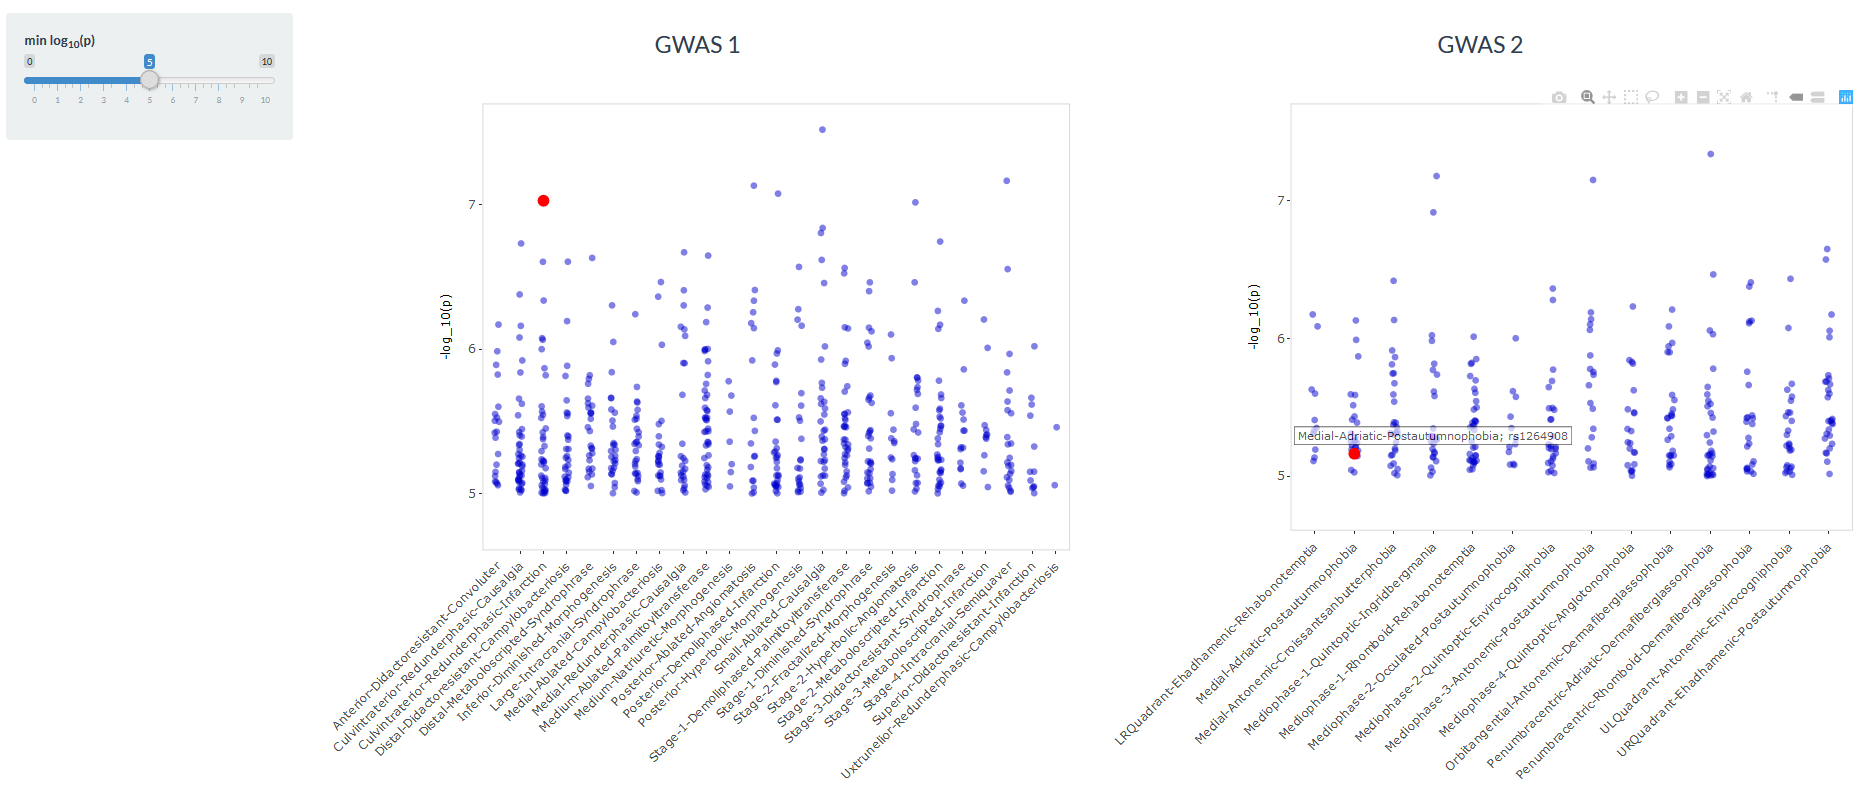
\includegraphics[width=6.5in, trim={0 0 0 0}, clip]{Tab1.png}
    \centering
    \caption{\texttt{plotly} pleiotropy app, tab 1, cross-GWAS phenotype SNP associations.}
    \label{fg:tab1}
\end{figure}


Important \texttt{plotly} features (numbers are lines in \texttt{Pleiotropy.r} source file):

\begin{itemize}
  \item (69) \texttt{geom\_jitter()}
  \item (85) Axis text angle
  \item (69) User defined variable in \texttt{aes()} for appearance in hover labels
  \item (151) Use of \texttt{plotly()} \%$>$\% to string function calls
  \item (380, 425) Use of \texttt{ggplotly()} to convert a \texttt{ggplot()} object to \texttt{plotly()}
  \item Hover label configuration (position and ID of aesthetics)
  \item (380, 388) Point selection and control of events
  \item (396) Subsetting observations for selected point
  \item (102) Coloring selected points using two geoms and data subsets in \texttt{t1ComposePlot2()}
  \item (411) Adding custom labels with \texttt{add\_annotations}, since \texttt{ggplotly()} does not convert them
  \item(420-425) Nested rendering of plots 
\end{itemize}

\clearpage

Figure \ref{fg:tab2} is an example screen shot of tab 2 of the pleiotropy app.  After filtering within-GWAS associations by significance (p), groups of inter-GWAS phenotypes are identified by clicking points in either set (left and right vertical blue dots).  Hovering over blue dots causes display of SNPs associated with a phenotype (within GWAS).  Hovering over a green dot (on an edge, or line connecting the GWAS sets) causes display of SNPs that are associated with the connected phenotypes (between GWAS). 

\begin{figure}[H]
    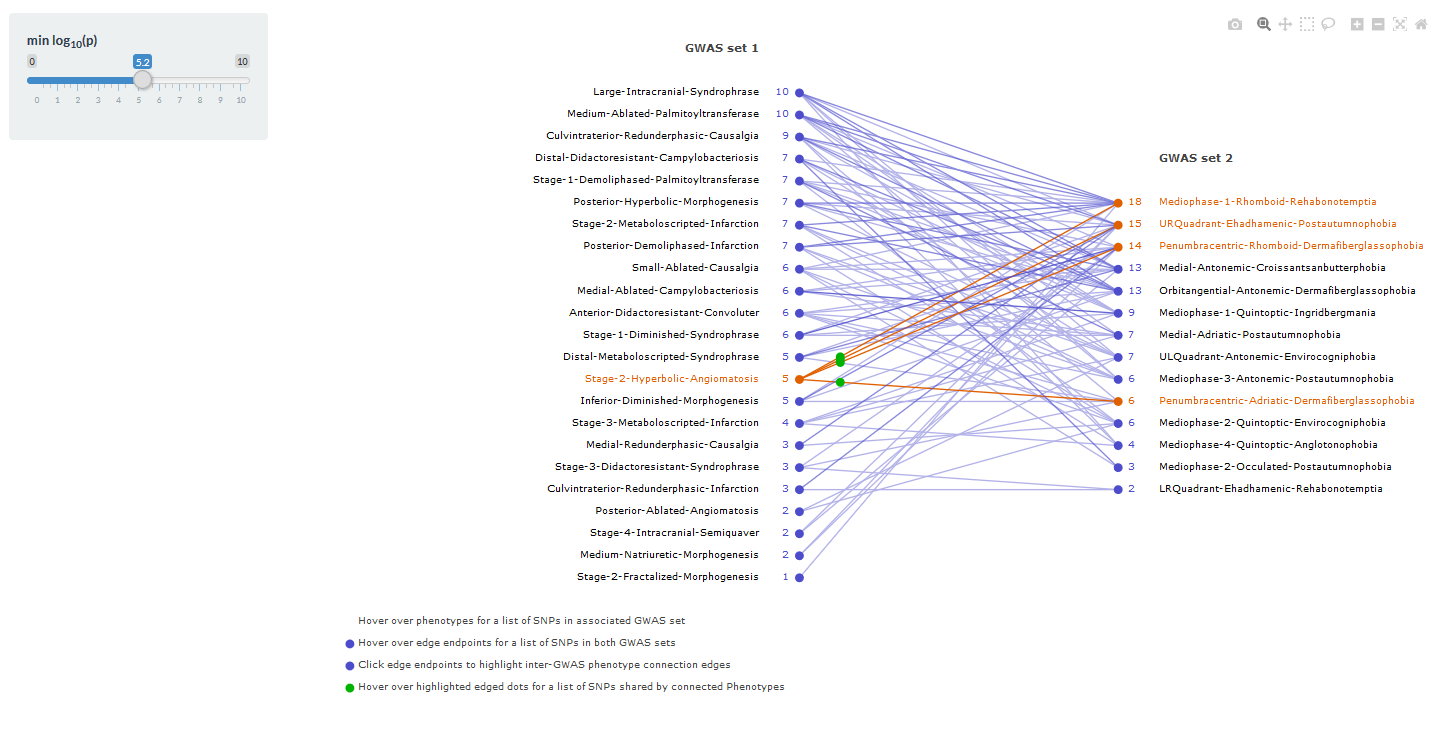
\includegraphics[width=6.5in, trim={0 0 0 0}, clip]{Tab2.png}
    \centering
    \caption{\texttt{plotly} pleiotropy app, tab 2, identification of phenotype association groups.  Associated SNPs appear as points are hovered over.}
    \label{fg:tab2}
\end{figure}

Important \texttt{plotly} features:

\begin{itemize}
    \item Subsetting plotted points by p-filter
    \item Phenotype ordering by number of associated SNPs
    \item Display of number of SNPs (\texttt{geom\_text()})
    \item Phenotype point hover labels
    \item Coloring vertices (phenotype) and edges (lines) of selected point (left and right)
    \item Display of green intersection point
    \item SNP intersection of lines, hover labels 
\end{itemize}

%%%%%%%%%%%%%%%%%%%%%%%%%%%%%%%%%%%%%%%%%%%%%%%%%%%%%%%%%%%%%%%%%%%%%%%%%%%%%%%%%%%%%%%%%%%%%%

\clearpage

\section{Debugging}\label{sec:debugging}

It is important that you have a means of communicating with your app during execution.  Unlike a typical R script, that can be executed one line at a time, with interactive review of variables, once a Shiny script launches, it executes without the console prompt.  Upon termination, some global variables may be available for examination, but you may not have reliable information on when they were last updated.  Error and warning messages are displayed in the console (and the terminal session when executed in a shell) and, fortunately, so are the results of \texttt{print()} and \texttt{cat()}.  When executed in RStudio, Shiny offers sophisticated debugger features (more info at \url{https://shiny.rstudio.com/articles/debugging.html}).  However, one of the simplest methods of communicating with your app during execution is to use \texttt{print()} (for a formatted or multi-element object, such as a data frame) or \texttt{cat(, file=stderr())} for ``small" objects.  The \texttt{file=stderr()} causes displayed items to appear in red.  Output may also be written to an error log, depending on your OS.  Considerations include

\begin{itemize}
    \item Shiny reports line numbers in error messages relative to the related function (\texttt{ui()} or \texttt{server()}) and, although not always exact, reported lines are usually in the proximity of the one which was executed at the time of error
    \item \texttt{cat("your message here")} displays in RStudio console (generally, consider Shiny Server)
    \item \texttt{cat("your message here", file=stderr())} is treated as an error (red in console, logged by OS)
    \item Messages appear in RStudio console when Shiny app launched from within RStudio
    \item Messages appear in terminal window when Shiny app launched with the \texttt{rscript} command in shell
    \item There exists a ``showcase" mode (\texttt{runApp(display.mode="showcase")}) that is intended to highlight each line of your script as it is executing
    \item The reactivity log may be helpful in debugging reactive sequencing issues (\texttt{options(shiny.reactlog=T)}, \url{https://shiny.rstudio.com/reference/shiny/0.14/showReactLog.html}
    \url It may be helpful to initially format an apps appearance with an empty \texttt{server()} function, then include executable statements once the screen objects are available and configured
    \item Although not strictly related to debugging, the use of \texttt{gc()} to clear defunct memory (from R's recycling) may reduce total memory in use at a given time
\end{itemize}


\end{spacing}

\end{document} 